% Options for packages loaded elsewhere
\PassOptionsToPackage{unicode}{hyperref}
\PassOptionsToPackage{hyphens}{url}
%
\documentclass[
]{book}
\usepackage{lmodern}
\usepackage{amsmath}
\usepackage{ifxetex,ifluatex}
\ifnum 0\ifxetex 1\fi\ifluatex 1\fi=0 % if pdftex
  \usepackage[T1]{fontenc}
  \usepackage[utf8]{inputenc}
  \usepackage{textcomp} % provide euro and other symbols
  \usepackage{amssymb}
\else % if luatex or xetex
  \usepackage{unicode-math}
  \defaultfontfeatures{Scale=MatchLowercase}
  \defaultfontfeatures[\rmfamily]{Ligatures=TeX,Scale=1}
\fi
% Use upquote if available, for straight quotes in verbatim environments
\IfFileExists{upquote.sty}{\usepackage{upquote}}{}
\IfFileExists{microtype.sty}{% use microtype if available
  \usepackage[]{microtype}
  \UseMicrotypeSet[protrusion]{basicmath} % disable protrusion for tt fonts
}{}
\makeatletter
\@ifundefined{KOMAClassName}{% if non-KOMA class
  \IfFileExists{parskip.sty}{%
    \usepackage{parskip}
  }{% else
    \setlength{\parindent}{0pt}
    \setlength{\parskip}{6pt plus 2pt minus 1pt}}
}{% if KOMA class
  \KOMAoptions{parskip=half}}
\makeatother
\usepackage{xcolor}
\IfFileExists{xurl.sty}{\usepackage{xurl}}{} % add URL line breaks if available
\IfFileExists{bookmark.sty}{\usepackage{bookmark}}{\usepackage{hyperref}}
\hypersetup{
  pdftitle={이원배치법: 자료와 분석에 대한 예제},
  pdfauthor={서울시립대 통계학과},
  hidelinks,
  pdfcreator={LaTeX via pandoc}}
\urlstyle{same} % disable monospaced font for URLs
\usepackage{color}
\usepackage{fancyvrb}
\newcommand{\VerbBar}{|}
\newcommand{\VERB}{\Verb[commandchars=\\\{\}]}
\DefineVerbatimEnvironment{Highlighting}{Verbatim}{commandchars=\\\{\}}
% Add ',fontsize=\small' for more characters per line
\usepackage{framed}
\definecolor{shadecolor}{RGB}{248,248,248}
\newenvironment{Shaded}{\begin{snugshade}}{\end{snugshade}}
\newcommand{\AlertTok}[1]{\textcolor[rgb]{0.94,0.16,0.16}{#1}}
\newcommand{\AnnotationTok}[1]{\textcolor[rgb]{0.56,0.35,0.01}{\textbf{\textit{#1}}}}
\newcommand{\AttributeTok}[1]{\textcolor[rgb]{0.77,0.63,0.00}{#1}}
\newcommand{\BaseNTok}[1]{\textcolor[rgb]{0.00,0.00,0.81}{#1}}
\newcommand{\BuiltInTok}[1]{#1}
\newcommand{\CharTok}[1]{\textcolor[rgb]{0.31,0.60,0.02}{#1}}
\newcommand{\CommentTok}[1]{\textcolor[rgb]{0.56,0.35,0.01}{\textit{#1}}}
\newcommand{\CommentVarTok}[1]{\textcolor[rgb]{0.56,0.35,0.01}{\textbf{\textit{#1}}}}
\newcommand{\ConstantTok}[1]{\textcolor[rgb]{0.00,0.00,0.00}{#1}}
\newcommand{\ControlFlowTok}[1]{\textcolor[rgb]{0.13,0.29,0.53}{\textbf{#1}}}
\newcommand{\DataTypeTok}[1]{\textcolor[rgb]{0.13,0.29,0.53}{#1}}
\newcommand{\DecValTok}[1]{\textcolor[rgb]{0.00,0.00,0.81}{#1}}
\newcommand{\DocumentationTok}[1]{\textcolor[rgb]{0.56,0.35,0.01}{\textbf{\textit{#1}}}}
\newcommand{\ErrorTok}[1]{\textcolor[rgb]{0.64,0.00,0.00}{\textbf{#1}}}
\newcommand{\ExtensionTok}[1]{#1}
\newcommand{\FloatTok}[1]{\textcolor[rgb]{0.00,0.00,0.81}{#1}}
\newcommand{\FunctionTok}[1]{\textcolor[rgb]{0.00,0.00,0.00}{#1}}
\newcommand{\ImportTok}[1]{#1}
\newcommand{\InformationTok}[1]{\textcolor[rgb]{0.56,0.35,0.01}{\textbf{\textit{#1}}}}
\newcommand{\KeywordTok}[1]{\textcolor[rgb]{0.13,0.29,0.53}{\textbf{#1}}}
\newcommand{\NormalTok}[1]{#1}
\newcommand{\OperatorTok}[1]{\textcolor[rgb]{0.81,0.36,0.00}{\textbf{#1}}}
\newcommand{\OtherTok}[1]{\textcolor[rgb]{0.56,0.35,0.01}{#1}}
\newcommand{\PreprocessorTok}[1]{\textcolor[rgb]{0.56,0.35,0.01}{\textit{#1}}}
\newcommand{\RegionMarkerTok}[1]{#1}
\newcommand{\SpecialCharTok}[1]{\textcolor[rgb]{0.00,0.00,0.00}{#1}}
\newcommand{\SpecialStringTok}[1]{\textcolor[rgb]{0.31,0.60,0.02}{#1}}
\newcommand{\StringTok}[1]{\textcolor[rgb]{0.31,0.60,0.02}{#1}}
\newcommand{\VariableTok}[1]{\textcolor[rgb]{0.00,0.00,0.00}{#1}}
\newcommand{\VerbatimStringTok}[1]{\textcolor[rgb]{0.31,0.60,0.02}{#1}}
\newcommand{\WarningTok}[1]{\textcolor[rgb]{0.56,0.35,0.01}{\textbf{\textit{#1}}}}
\usepackage{longtable,booktabs}
\usepackage{calc} % for calculating minipage widths
% Correct order of tables after \paragraph or \subparagraph
\usepackage{etoolbox}
\makeatletter
\patchcmd\longtable{\par}{\if@noskipsec\mbox{}\fi\par}{}{}
\makeatother
% Allow footnotes in longtable head/foot
\IfFileExists{footnotehyper.sty}{\usepackage{footnotehyper}}{\usepackage{footnote}}
\makesavenoteenv{longtable}
\usepackage{graphicx}
\makeatletter
\def\maxwidth{\ifdim\Gin@nat@width>\linewidth\linewidth\else\Gin@nat@width\fi}
\def\maxheight{\ifdim\Gin@nat@height>\textheight\textheight\else\Gin@nat@height\fi}
\makeatother
% Scale images if necessary, so that they will not overflow the page
% margins by default, and it is still possible to overwrite the defaults
% using explicit options in \includegraphics[width, height, ...]{}
\setkeys{Gin}{width=\maxwidth,height=\maxheight,keepaspectratio}
% Set default figure placement to htbp
\makeatletter
\def\fps@figure{htbp}
\makeatother
\setlength{\emergencystretch}{3em} % prevent overfull lines
\providecommand{\tightlist}{%
  \setlength{\itemsep}{0pt}\setlength{\parskip}{0pt}}
\setcounter{secnumdepth}{5}
\usepackage[onehalfspacing]{setspace}

\usepackage[hangul]{kotex}
\newcommand{\pardiff}[2]{\frac{\partial #1}{\partial #2 }}
\newcommand{\pardiffl}[2]{{\partial #1}/{\partial #2 }}
\newcommand{\pardiffd}[2]{\frac{\partial^2 #1}{\partial #2^t \partial #2 }}
\newcommand{\pardiffdd}[3]{\frac{\partial^2 #1}{\partial #2 \partial #3 }}

\newcommand{\bm}[1]{ \symbf{#1}}

\usepackage{booktabs}
\usepackage{longtable}
\usepackage[bf,singlelinecheck=off]{caption}

%\setmainfont[UprightFeatures={SmallCapsFont=AlegreyaSC-Regular}]{Alegreya}

\usepackage{framed,color}
\definecolor{shadecolor}{RGB}{248,248,248}

\renewcommand{\textfraction}{0.05}
\renewcommand{\topfraction}{0.8}
\renewcommand{\bottomfraction}{0.8}
\renewcommand{\floatpagefraction}{0.75}

\renewenvironment{quote}{\begin{VF}}{\end{VF}}
\let\oldhref\href
\renewcommand{\href}[2]{#2\footnote{\url{#1}}}

\makeatletter
\newenvironment{kframe}{%
\medskip{}
\setlength{\fboxsep}{.8em}
 \def\at@end@of@kframe{}%
 \ifinner\ifhmode%
  \def\at@end@of@kframe{\end{minipage}}%
  \begin{minipage}{\columnwidth}%
 \fi\fi%
 \def\FrameCommand##1{\hskip\@totalleftmargin \hskip-\fboxsep
 \colorbox{shadecolor}{##1}\hskip-\fboxsep
     % There is no \\@totalrightmargin, so:
     \hskip-\linewidth \hskip-\@totalleftmargin \hskip\columnwidth}%
 \MakeFramed {\advance\hsize-\width
   \@totalleftmargin\z@ \linewidth\hsize
   \@setminipage}}%
 {\par\unskip\endMakeFramed%
 \at@end@of@kframe}
\makeatother

\makeatletter

\@ifundefined{Shaded}{
}{\renewenvironment{Shaded}{\begin{kframe}}{\end{kframe}}}
\makeatother

\newenvironment{rmdblock}[1]
  {
  \begin{itemize}
  \renewcommand{\labelitemi}{
    \raisebox{-.7\height}[0pt][0pt]{
      {\setkeys{Gin}{width=3em,keepaspectratio}\includegraphics{images/#1}}
    }
  }
  \setlength{\fboxsep}{1em}
  \begin{kframe}
  \item
  }
  {
  \end{kframe}
  \end{itemize}
  }
  
\newenvironment{rmdnote}
  {\begin{rmdblock}{note}}
  {\end{rmdblock}}
  
\newenvironment{rmdcaution}
  {\begin{rmdblock}{caution}}
  {\end{rmdblock}}
  
\newenvironment{rmdimportant}
  {\begin{rmdblock}{important}}
  {\end{rmdblock}}
  
\newenvironment{rmdtip}
  {\begin{rmdblock}{tip}}
  {\end{rmdblock}}
  
\newenvironment{rmdwarning}
  {\begin{rmdblock}{warning}}
  {\end{rmdblock}}
  


%\usepackage{makeidx}
%\makeindex

\urlstyle{tt}

\usepackage{amsthm}
\makeatletter
 \def\thm@space@setup{%
   \thm@preskip=8pt plus 2pt minus 4pt
   \thm@postskip=\thm@preskip
}
\makeatother

\frontmatter

\ifluatex
  \usepackage{selnolig}  % disable illegal ligatures
\fi
\usepackage[]{natbib}
\bibliographystyle{apalike}

\title{이원배치법: 자료와 분석에 대한 예제}
\author{서울시립대 통계학과}
\date{2021-03-23}

\begin{document}
\maketitle

{
\setcounter{tocdepth}{1}
\tableofcontents
}
\hypertarget{uxc11cuxbb38}{%
\chapter*{서문}\label{uxc11cuxbb38}}


이원배치법에 대한 예제, R 프로그램과 결과 해석에 대한 강의자료입니다.

이 노트에 있는 R 프로그램을 실행하려면 다음과 같은 패키지들이 필요하다.

\begin{verbatim}
library(dplyr)
library(tidyr)
library(ggplot2)
library(ggbeeswarm)
library(MontgomeryDAE)
library(emmeans)
\end{verbatim}

\mainmatter

\hypertarget{battery}{%
\chapter{전지의 수명 실험}\label{battery}}

전지(battery)를 제조하는 회사의 기술자들이 전지의 수명(\texttt{BatteryLife})에 영향을 미치는 두 요인, 온도(\texttt{Temperature})와 재료(\texttt{MaterialType})의 효과를 알아보기 위해서 실행한 실험입니다.

기술자들은 온도가 크게 변할 때 전지의 수명에 어떤 영향을 미치는지 알아보기 위하여 실험을 실시하였다. 온도는 3개의 수준(15도, 70도, 125도)을 고려하였다. 전지를 생산하는 재료가 3개이므로 재료는 3개의 수준(type 1,2,3)으로 구성되어 있다. 이 실험은 9 개의 처리(\(ab=3\times 3=9\))에 대하여 각각 4번의 반복 측정(\(r=4\))을 실시하였다.

자료의 출처는 \citep{montgomery2017design} 에 나와 있다

자료를 얻기 위해서는 다음과 같은 R 프로그램을 실행하여 패키지 \texttt{MontgomeryDAE}를 설치하고 실행해야 한다.

\begin{Shaded}
\begin{Highlighting}[]
\FunctionTok{install.packages}\NormalTok{(}\StringTok{"remotes"}\NormalTok{)}
\NormalTok{remotes}\SpecialCharTok{::}\FunctionTok{install\_github}\NormalTok{(}\StringTok{"ehassler/MontgomeryDAE"}\NormalTok{)}
\FunctionTok{library}\NormalTok{(MontgomeryDAE)}
\end{Highlighting}
\end{Shaded}

\hypertarget{uxc790uxb8cc-uxc77duxae30}{%
\section{자료 읽기}\label{uxc790uxb8cc-uxc77duxae30}}

이제 전지의 수명 실험 자료를 읽어 오자. 전지의 수명 실험에 대한 자료는 데이터프레임 \texttt{Table5.1}에 있다.

\begin{Shaded}
\begin{Highlighting}[]
\NormalTok{df }\OtherTok{\textless{}{-}}\NormalTok{ Table5}\FloatTok{.1}
\FunctionTok{head}\NormalTok{(df) }\CommentTok{\# 자료의 앞부부만 보기   }
\end{Highlighting}
\end{Shaded}

\begin{verbatim}
##   MaterialType Temperature BatteryLife
## 1            1          15         130
## 2            1          15          74
## 3            2          15         150
## 4            2          15         159
## 5            3          15         138
## 6            3          15         168
\end{verbatim}

함수 \texttt{str()}은 자료의 구조와 자료 안에 있는 변수의 형식을 보여준다.

\begin{Shaded}
\begin{Highlighting}[]
\FunctionTok{str}\NormalTok{(df)  }\CommentTok{\# 자료의 구조를 알아보는 명령}
\end{Highlighting}
\end{Shaded}

\begin{verbatim}
## 'data.frame':    36 obs. of  3 variables:
##  $ MaterialType: chr  "1" "1" "2" "2" ...
##  $ Temperature : num  15 15 15 15 15 15 15 15 15 15 ...
##  $ BatteryLife : num  130 74 150 159 138 168 155 180 188 126 ...
\end{verbatim}

위의 결과를 보면 데이터프레임 \texttt{df}에 있는 변수 \texttt{MaterialType}은 문자형 변수(\texttt{chr})이고 나머지는 숫자형 변수(\texttt{num})이다. 두 요인에 대한 변수인 \texttt{MaterialType}와 \texttt{Temperature}를 함수 \texttt{factor()}를 이용하여 범주형 변수로 만들어 주자 .

\begin{Shaded}
\begin{Highlighting}[]
\NormalTok{df}\SpecialCharTok{$}\NormalTok{MaterialType }\OtherTok{\textless{}{-}} \FunctionTok{factor}\NormalTok{(df}\SpecialCharTok{$}\NormalTok{MaterialType)}
\NormalTok{df}\SpecialCharTok{$}\NormalTok{Temperature }\OtherTok{\textless{}{-}} \FunctionTok{factor}\NormalTok{(df}\SpecialCharTok{$}\NormalTok{Temperature)}
\FunctionTok{str}\NormalTok{(df)}
\end{Highlighting}
\end{Shaded}

\begin{verbatim}
## 'data.frame':    36 obs. of  3 variables:
##  $ MaterialType: Factor w/ 3 levels "1","2","3": 1 1 2 2 3 3 1 1 2 2 ...
##  $ Temperature : Factor w/ 3 levels "15","70","125": 1 1 1 1 1 1 1 1 1 1 ...
##  $ BatteryLife : num  130 74 150 159 138 168 155 180 188 126 ...
\end{verbatim}

\hypertarget{uxc790uxb8ccuxc758-uxc2dcuxac01uxd654uxc640-uxae30uxcd08-uxd1b5uxacc4uxb7c9}{%
\section{자료의 시각화와 기초 통계량}\label{uxc790uxb8ccuxc758-uxc2dcuxac01uxd654uxc640-uxae30uxcd08-uxd1b5uxacc4uxb7c9}}

이제 처리별로 효과를 시각적으로 비교하기 위하여 자료들에 대한 산점도와 상자그림을 그려보자

\begin{Shaded}
\begin{Highlighting}[]
\NormalTok{df }\SpecialCharTok{\%\textgreater{}\%} 
  \FunctionTok{ggplot}\NormalTok{() }\SpecialCharTok{+}
  \FunctionTok{aes}\NormalTok{(}\AttributeTok{x =}\NormalTok{ Temperature , }\AttributeTok{y =}\NormalTok{ BatteryLife, }\AttributeTok{fill=}\NormalTok{MaterialType, }\AttributeTok{color=}\NormalTok{MaterialType, }\AttributeTok{group =} \FunctionTok{interaction}\NormalTok{(Temperature, MaterialType)) }\SpecialCharTok{+}
  \FunctionTok{geom\_boxplot}\NormalTok{(}\AttributeTok{alpha =} \FloatTok{0.1}\NormalTok{, }\AttributeTok{width =} \FloatTok{0.75}\NormalTok{) }\SpecialCharTok{+}
  \FunctionTok{geom\_beeswarm}\NormalTok{(}\AttributeTok{dodge.width =} \FloatTok{0.75}\NormalTok{)}
\end{Highlighting}
\end{Shaded}

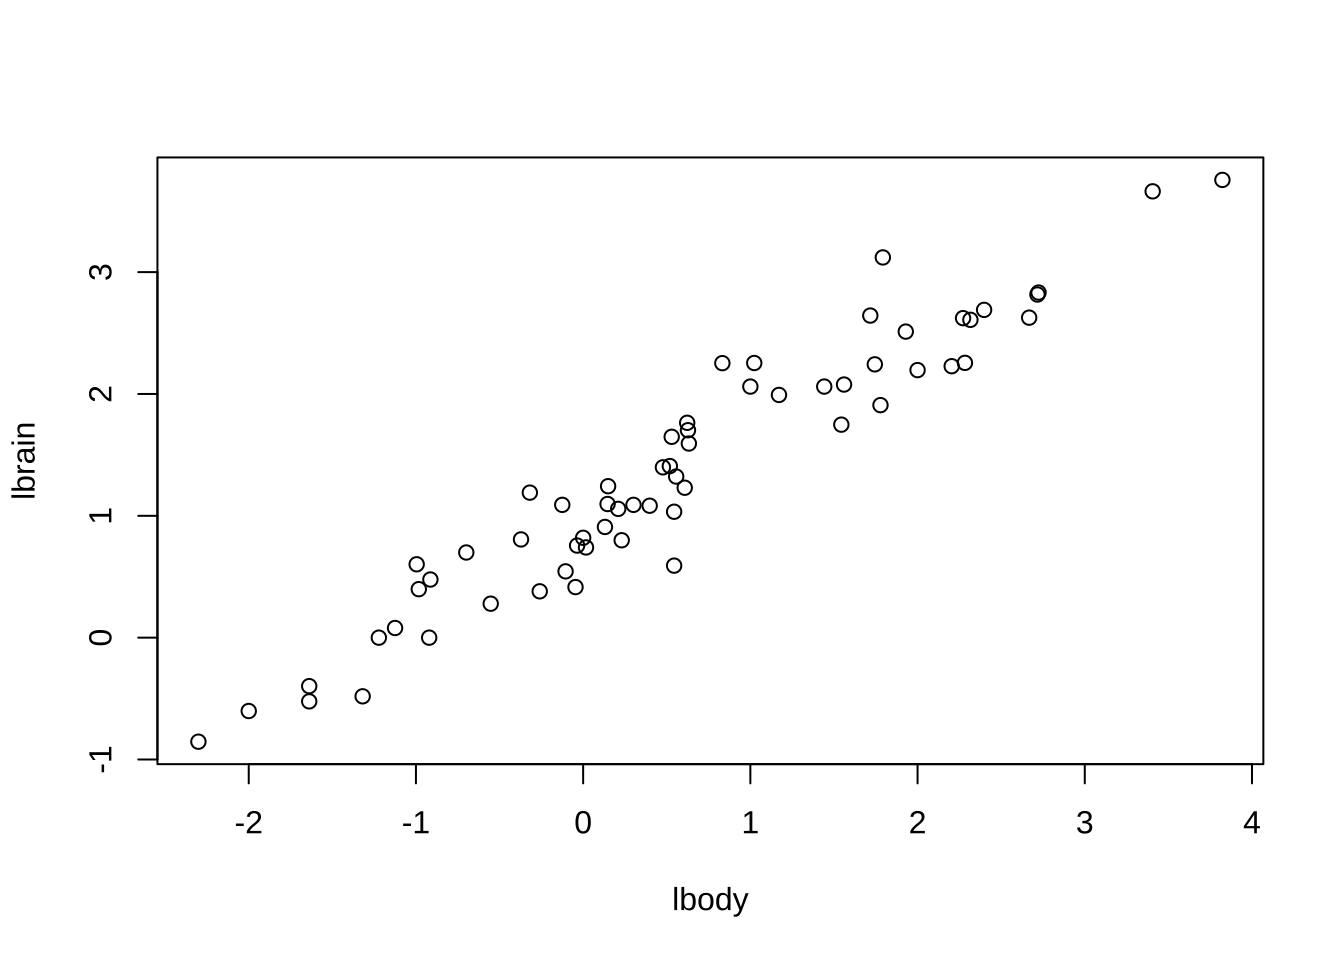
\includegraphics{Two-way-ANOVA_files/figure-latex/unnamed-chunk-6-1.pdf}

다음으로 6개의 처리 조합에 대한 전지 수명의 기초통계량(평균과 표준편차)을 구해보자.

\begin{Shaded}
\begin{Highlighting}[]
\NormalTok{dfs }\OtherTok{\textless{}{-}}\NormalTok{ df }\SpecialCharTok{\%\textgreater{}\%} \FunctionTok{group\_by}\NormalTok{(MaterialType, Temperature)  }\SpecialCharTok{\%\textgreater{}\%}  \FunctionTok{summarise}\NormalTok{(}\AttributeTok{mean=}\FunctionTok{mean}\NormalTok{(BatteryLife),  }\AttributeTok{sd=}\FunctionTok{sd}\NormalTok{(BatteryLife))}
\end{Highlighting}
\end{Shaded}

\begin{verbatim}
## `summarise()` has grouped output by 'MaterialType'. You can override using the `.groups` argument.
\end{verbatim}

\begin{Shaded}
\begin{Highlighting}[]
\NormalTok{dfs}
\end{Highlighting}
\end{Shaded}

\begin{verbatim}
## # A tibble: 9 x 4
## # Groups:   MaterialType [3]
##   MaterialType Temperature  mean    sd
##   <fct>        <fct>       <dbl> <dbl>
## 1 1            15          135.   45.4
## 2 1            70           57.2  23.6
## 3 1            125          57.5  26.9
## 4 2            15          156.   25.6
## 5 2            70          120.   12.7
## 6 2            125          49.5  19.3
## 7 3            15          144    26.0
## 8 3            70          146.   22.5
## 9 3            125          85.5  19.3
\end{verbatim}

이제 위에서 계산된 처리 그룹에 대한 평균으로 상호작용 그림을 그려보자. 아래 그림에서 온도가 증가할 수록 전지의 수명이 감소하는 경향을 보이고 있다. 또한 각 재료에 따른 온도의 변화가 수평으로 나타나지 않고 있음을 알 수 있다. 이러한 점은 온도와 재료 사이에 유의한 상호작용이 있다고 예측할 수 있다.

\begin{Shaded}
\begin{Highlighting}[]
\NormalTok{dfs }\SpecialCharTok{\%\textgreater{}\%} 
  \FunctionTok{ggplot}\NormalTok{() }\SpecialCharTok{+}
  \FunctionTok{aes}\NormalTok{(}\AttributeTok{x =}\NormalTok{ Temperature , }\AttributeTok{y =}\NormalTok{ mean, }\AttributeTok{color =}\NormalTok{MaterialType) }\SpecialCharTok{+}
  \FunctionTok{geom\_line}\NormalTok{(}\FunctionTok{aes}\NormalTok{(}\AttributeTok{group =}\NormalTok{ MaterialType)) }\SpecialCharTok{+}
  \FunctionTok{geom\_point}\NormalTok{()}
\end{Highlighting}
\end{Shaded}

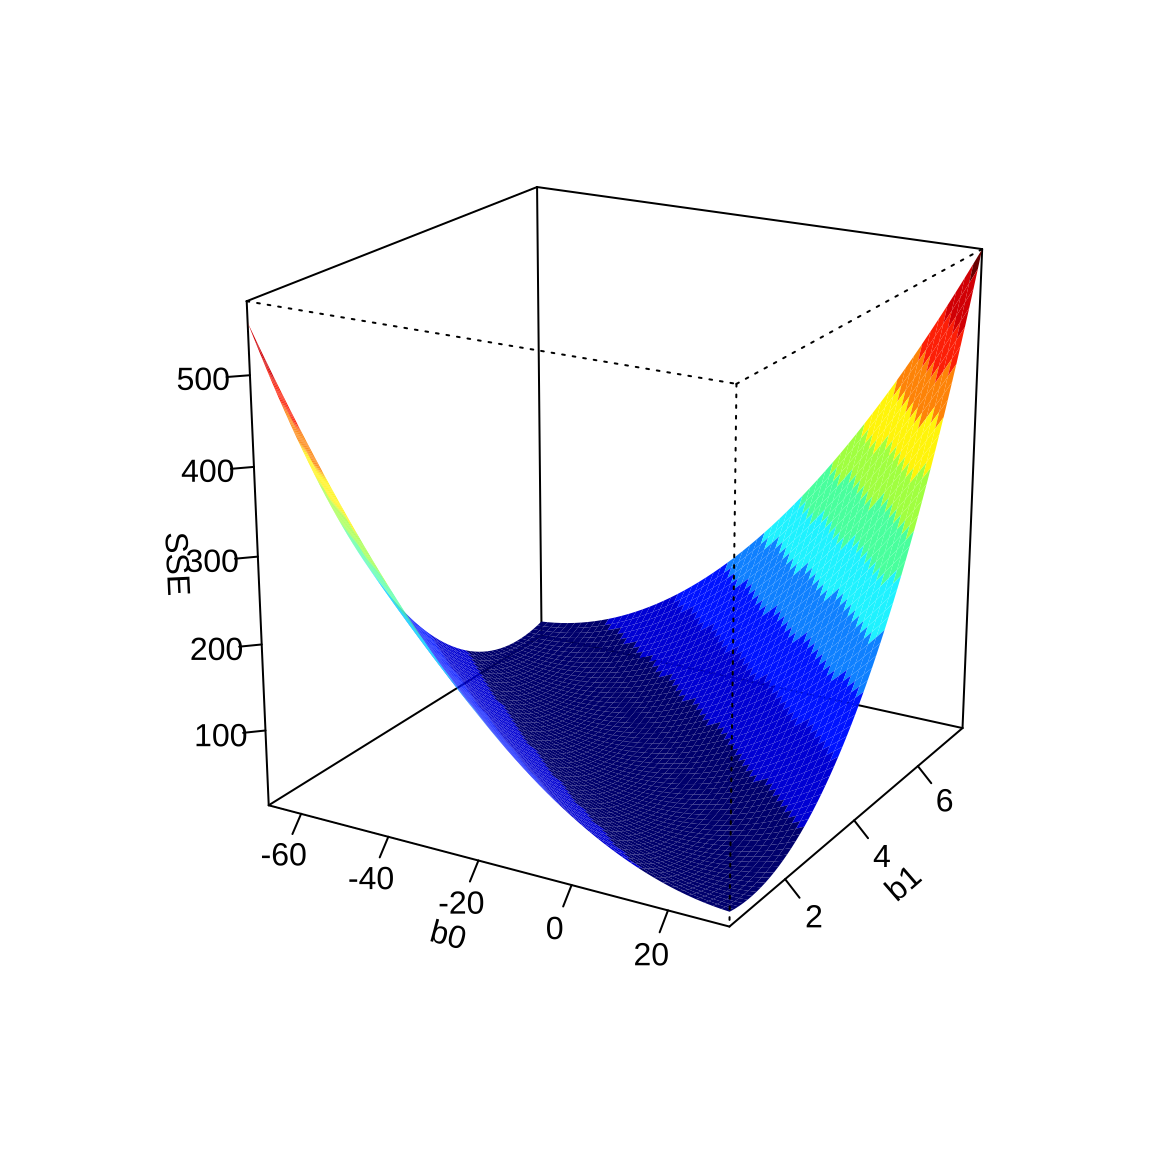
\includegraphics{Two-way-ANOVA_files/figure-latex/unnamed-chunk-8-1.pdf}

\hypertarget{uxbd84uxc0b0uxbd84uxc11duxd45cuxc640-uxac00uxc124uxac80uxc815}{%
\section{분산분석표와 가설검정}\label{uxbd84uxc0b0uxbd84uxc11duxd45cuxc640-uxac00uxc124uxac80uxc815}}

이제 다음과 같은 모형에서 이원배치법에서의 가설검정을 수행하기 위하여 분산분석 표를 구해보자.

\[ x_{ijk} = \mu + \alpha_i + \beta_j + (\alpha\beta)_{ij} + e_{ijk} \]

\begin{longtable}[]{@{}crrrc@{}}
\toprule
\begin{minipage}[b]{(\columnwidth - 4\tabcolsep) * \real{0.24}}\centering
요인\strut
\end{minipage} & \begin{minipage}[b]{(\columnwidth - 4\tabcolsep) * \real{0.10}}\raggedleft
제곱합\strut
\end{minipage} & \begin{minipage}[b]{(\columnwidth - 4\tabcolsep) * \real{0.25}}\raggedleft
자유도\strut
\end{minipage} & \begin{minipage}[b]{(\columnwidth - 4\tabcolsep) * \real{0.25}}\raggedleft
평균제곱합\strut
\end{minipage} & \begin{minipage}[b]{(\columnwidth - 4\tabcolsep) * \real{0.15}}\centering
\(F_0\)\strut
\end{minipage}\tabularnewline
\midrule
\endhead
\begin{minipage}[t]{(\columnwidth - 4\tabcolsep) * \real{0.24}}\centering
요인 \(A\)\strut
\end{minipage} & \begin{minipage}[t]{(\columnwidth - 4\tabcolsep) * \real{0.10}}\raggedleft
\(SS_A\)\strut
\end{minipage} & \begin{minipage}[t]{(\columnwidth - 4\tabcolsep) * \real{0.25}}\raggedleft
\(a-1\)\strut
\end{minipage} & \begin{minipage}[t]{(\columnwidth - 4\tabcolsep) * \real{0.25}}\raggedleft
\(MS_A\)\strut
\end{minipage} & \begin{minipage}[t]{(\columnwidth - 4\tabcolsep) * \real{0.15}}\centering
\(MS_A/MS_E\)\strut
\end{minipage}\tabularnewline
\begin{minipage}[t]{(\columnwidth - 4\tabcolsep) * \real{0.24}}\centering
요인 \(B\)\strut
\end{minipage} & \begin{minipage}[t]{(\columnwidth - 4\tabcolsep) * \real{0.10}}\raggedleft
\(SS_B\)\strut
\end{minipage} & \begin{minipage}[t]{(\columnwidth - 4\tabcolsep) * \real{0.25}}\raggedleft
\(b-1\)\strut
\end{minipage} & \begin{minipage}[t]{(\columnwidth - 4\tabcolsep) * \real{0.25}}\raggedleft
\(MS_B\)\strut
\end{minipage} & \begin{minipage}[t]{(\columnwidth - 4\tabcolsep) * \real{0.15}}\centering
\(MS_B/MS_E\)\strut
\end{minipage}\tabularnewline
\begin{minipage}[t]{(\columnwidth - 4\tabcolsep) * \real{0.24}}\centering
상호작용 \(A \times B\)\strut
\end{minipage} & \begin{minipage}[t]{(\columnwidth - 4\tabcolsep) * \real{0.10}}\raggedleft
\(SS_{A \times B}\)\strut
\end{minipage} & \begin{minipage}[t]{(\columnwidth - 4\tabcolsep) * \real{0.25}}\raggedleft
\((a-1)(b-1)\)\strut
\end{minipage} & \begin{minipage}[t]{(\columnwidth - 4\tabcolsep) * \real{0.25}}\raggedleft
\(MS_{A \times B}\)\strut
\end{minipage} & \begin{minipage}[t]{(\columnwidth - 4\tabcolsep) * \real{0.15}}\centering
\(MS_{A \times B}/MS_E\)\strut
\end{minipage}\tabularnewline
\begin{minipage}[t]{(\columnwidth - 4\tabcolsep) * \real{0.24}}\centering
잔차 \(E\)\strut
\end{minipage} & \begin{minipage}[t]{(\columnwidth - 4\tabcolsep) * \real{0.10}}\raggedleft
\(SS_E\)\strut
\end{minipage} & \begin{minipage}[t]{(\columnwidth - 4\tabcolsep) * \real{0.25}}\raggedleft
\(ab(r-1)\)\strut
\end{minipage} & \begin{minipage}[t]{(\columnwidth - 4\tabcolsep) * \real{0.25}}\raggedleft
\(MS_E\)\strut
\end{minipage} & \begin{minipage}[t]{(\columnwidth - 4\tabcolsep) * \real{0.15}}\centering
\strut
\end{minipage}\tabularnewline
\begin{minipage}[t]{(\columnwidth - 4\tabcolsep) * \real{0.24}}\centering
총합\strut
\end{minipage} & \begin{minipage}[t]{(\columnwidth - 4\tabcolsep) * \real{0.10}}\raggedleft
\(SS_T\)\strut
\end{minipage} & \begin{minipage}[t]{(\columnwidth - 4\tabcolsep) * \real{0.25}}\raggedleft
\(abr-1\)\strut
\end{minipage} & \begin{minipage}[t]{(\columnwidth - 4\tabcolsep) * \real{0.25}}\raggedleft
\strut
\end{minipage} & \begin{minipage}[t]{(\columnwidth - 4\tabcolsep) * \real{0.15}}\centering
\strut
\end{minipage}\tabularnewline
\bottomrule
\end{longtable}

\begin{Shaded}
\begin{Highlighting}[]
\NormalTok{dfaov }\OtherTok{\textless{}{-}} \FunctionTok{aov}\NormalTok{(BatteryLife}\SpecialCharTok{\textasciitilde{}}\NormalTok{ MaterialType }\SpecialCharTok{+}\NormalTok{ Temperature }\SpecialCharTok{+}\NormalTok{ MaterialType}\SpecialCharTok{:}\NormalTok{Temperature, }\AttributeTok{data=}\NormalTok{df)}
\CommentTok{\# This is equivalent to aov(BatteryLife\textasciitilde{} MaterialType *Temperature , data=df)}
\FunctionTok{summary}\NormalTok{(dfaov)}
\end{Highlighting}
\end{Shaded}

\begin{verbatim}
##                          Df Sum Sq Mean Sq F value   Pr(>F)    
## MaterialType              2  10684    5342   7.911  0.00198 ** 
## Temperature               2  39119   19559  28.968 1.91e-07 ***
## MaterialType:Temperature  4   9614    2403   3.560  0.01861 *  
## Residuals                27  18231     675                     
## ---
## Signif. codes:  0 '***' 0.001 '**' 0.01 '*' 0.05 '.' 0.1 ' ' 1
\end{verbatim}

\begin{itemize}
\item
  상호작용에 대한 가설 검정
  \[ H_0: (\alpha \beta)_{11} = (\alpha \beta)_{12} =\cdots = (\alpha \beta)_{3,3} =0 \quad \text{ vs.} \quad H_1: \text{ not } H_0 \]

  분산분석표에서 상호작용에 대한 가설 검정을 위한 F-통계량은 다음과 같다.

  \[ F_0 = \frac{MS_{A \times B}}{MS_E} =\frac{SS_{A\times B}/\phi_{AB}} {SS_E/\phi_E} = \frac{9614/4}{18231/27} = 3.560 \]

  위의 F-통계량에 대한 p-값은 0.0186으로 유의수준 0.05보다 작으므로 귀무가설 \(H_0\)를 기각한다. 따라서 온도와 재료의 상호작용은 유의하다.
\item
  주효과에 대한 가설 검정

  위에서 유의한 상호작용이 있다고 판단하였기 때문에 주효과에 대한 가설검정은 기술적 의미가 없다. 기술적으로 의미가 없다는 것은 유의한 상호작용이 있으면 이미 주효과 \(A\) 의크기가 \(B\) 의 수준에 따라서 다르므로 주효과가 유의하게 있다는 것을 뜻한다.
\end{itemize}

\hypertarget{uxbd84uxc0b0uxbd84uxc11d-uxd6c4uxc758-uxcd94uxc815}{%
\section{분산분석 후의 추정}\label{uxbd84uxc0b0uxbd84uxc11d-uxd6c4uxc758-uxcd94uxc815}}

\hypertarget{uxbaa8uxd3c9uxade0uxc5d0-uxb300uxd55c-uxcd94uxb860}{%
\subsection{모평균에 대한 추론}\label{uxbaa8uxd3c9uxade0uxc5d0-uxb300uxd55c-uxcd94uxb860}}

이원배치에서 유의한 상호작용이 있는 경우 처리수준 \(A_iB_j\)에 대한 모평균 \(\mu_{ij}\) 은 다음과 같다.

\[ \mu_{ij} = \mu + \alpha_i + \beta_j + (\alpha \beta)_{ij} = \mu + \tau_{ij} \]

이때 \(\mu_{ij}\) 에 대한 추정량은 처리수준 \(A_iB_j\)에서의 관측값들의 평균 \(\bar {x}_{ij.}\)으로 다음과 같은 분포를 따른다.

\[ \bar {x}_{ij.} \sim N(\mu_{ij}, \sigma^2_E/ r) \]

오차항의 분산 \(\sigma^2_E\)는 분산분석표에서 \(MS_E\)로 추정할 수 있다.

\[ \hat \sigma^2_E = MS_E = \frac{SS_E}{ab(r-1)} =\frac{18231}{27} = 675 \]

위의 결과를 이용하면 처리수준 \(A_iB_j\)에 대한 모평균 \(\mu_{ij}\)에 대한 \(100(1-\alpha)\)\% 신뢰구간은 다음과 같이 주어진다.

\[ \bar x_{ij.} \pm t(1-\alpha/2, ab[r-1]) \sqrt{ \frac{MS_E}{r}}  \]

예를 들어 전지의 수명실험에서 온도가 70도이고(\(i=2\)) 재료의 형테가 3인 경우(\(j=3\)) 수명 시간의 평균 \(\mu_{23}\) 에 대한 95\% 신뢰 구간을 구해보자. 일단 위의 기초 통계량에서 \(\bar x_{13.}=146\) 이고 분산분석표에서 \(MS_E =675\), \(r=4\) 그리고 t-분포의 백분위수 \(t(0.975, 27)\) 은 다음과 같이 주어진다.

\begin{Shaded}
\begin{Highlighting}[]
\FunctionTok{qt}\NormalTok{(}\FloatTok{0.975}\NormalTok{, }\DecValTok{27}\NormalTok{)}
\end{Highlighting}
\end{Shaded}

\begin{verbatim}
## [1] 2.051831
\end{verbatim}

따라서 \(\mu_{23}\) 에 대한 95\% 신뢰 구간은 다음과 같다.

\[ \bar x_{23.} \pm t(1-\alpha/2, ab[r-1]) \sqrt{ \frac{MS_E}{r}} = 146 \pm (2.05)\sqrt{\frac{675}{4}} = (119, 172) \]

패키지 \texttt{emmeans}에 있는 함수 \texttt{emmeans()}를 다음과 같이 사용하면 각 처리에 대한 평균의 95\% 신뢰구간을 쉽게 구할 수 있다. 함수 \texttt{emmeans()}의 첫 번째 인자는 분산분석의 결과(\texttt{aov()}의 결과)이며 다음의 인자들은 요인에 대한 변수명을 써주면 된다.

\begin{Shaded}
\begin{Highlighting}[]
\FunctionTok{emmeans}\NormalTok{(dfaov, }\StringTok{"MaterialType"}\NormalTok{,}\StringTok{"Temperature"}\NormalTok{)}
\end{Highlighting}
\end{Shaded}

\begin{verbatim}
## Temperature = 15:
##  MaterialType emmean SE df lower.CL upper.CL
##  1             134.8 13 27    108.1    161.4
##  2             155.8 13 27    129.1    182.4
##  3             144.0 13 27    117.3    170.7
## 
## Temperature = 70:
##  MaterialType emmean SE df lower.CL upper.CL
##  1              57.2 13 27     30.6     83.9
##  2             119.8 13 27     93.1    146.4
##  3             145.8 13 27    119.1    172.4
## 
## Temperature = 125:
##  MaterialType emmean SE df lower.CL upper.CL
##  1              57.5 13 27     30.8     84.2
##  2              49.5 13 27     22.8     76.2
##  3              85.5 13 27     58.8    112.2
## 
## Confidence level used: 0.95
\end{verbatim}

함수 \texttt{emmeans()}에서 출력되는 \texttt{SE}는 표분오차(standard error)를 의미하며 이는 평균의 추정량 \(\bar x_{ij.}\)의 표준편차(standard deviation)이다.

\[  \hat{\text{SE}}(\bar x_{ij.}) = \hat{ sd} (\bar x_{ij.}) = \sqrt{ \hat {Var} (\bar x_{ij.})}
= \sqrt{\frac{MS_E}{r}} = \sqrt{675/4} = 13.0 \]

\hypertarget{uxbbf8uxb798uxc758-uxad00uxce21uxac12uxc5d0-uxb300uxd55c-uxcd94uxb860}{%
\section{미래의 관측값에 대한 추론}\label{uxbbf8uxb798uxc758-uxad00uxce21uxac12uxc5d0-uxb300uxd55c-uxcd94uxb860}}

처리수준 \(A_iB_j\)에 대한 미래의 관측값에 대한 신뢰구간을 구하는 경우 관측 오차에 의한 불확실성을 반영하기 때문에 그 신뢰구간은 다음과 같이 주어진다.

\[ \bar x_{ij.} \pm t(1-\alpha/2, ab[r-1]) \sqrt{ \frac{MS_E}{r}+MS_E}  \]

참고로 다른 교과서에서는 관측값에 대한 신뢰구간을 예측구간(prediction interval)이라고 부른다. 이는 모수는 추정(estimation)하지만 관측값은 예측(prediction)한다고 말하기 때문이다.

\hypertarget{ex41}{%
\chapter{예제 4.1}\label{ex41}}

예제 4.1 은 교과서 89 페이지에 나온 분석 예제이다. 4종류의 사료(A)와 3종류의 돼지품종(B)이 체중 증가에 미치는 영향을 조사한 실험이다. 각 처리 조합마다 3회 반복실험하여 총 36개의 관측값을 얻었다.

\hypertarget{uxc790uxb8cc-uxc77duxae30-1}{%
\section{자료 읽기}\label{uxc790uxb8cc-uxc77duxae30-1}}

다음과 같은 순서로 자료를 가진 데이터프레임 \texttt{df2}을 만들어 보자.

\begin{Shaded}
\begin{Highlighting}[]
\NormalTok{response}\OtherTok{\textless{}{-}} \FunctionTok{c}\NormalTok{(}\DecValTok{64}\NormalTok{, }\DecValTok{66}\NormalTok{, }\DecValTok{70}\NormalTok{, }\DecValTok{72}\NormalTok{, }\DecValTok{81}\NormalTok{, }\DecValTok{64}\NormalTok{, }
             \DecValTok{74}\NormalTok{, }\DecValTok{51}\NormalTok{, }\DecValTok{65}\NormalTok{, }\DecValTok{65}\NormalTok{, }\DecValTok{63}\NormalTok{, }\DecValTok{58}\NormalTok{,}
             \DecValTok{57}\NormalTok{, }\DecValTok{43}\NormalTok{, }\DecValTok{52}\NormalTok{, }\DecValTok{47}\NormalTok{, }\DecValTok{58}\NormalTok{, }\DecValTok{67}\NormalTok{,}
             \DecValTok{59}\NormalTok{, }\DecValTok{68}\NormalTok{, }\DecValTok{65}\NormalTok{, }\DecValTok{66}\NormalTok{, }\DecValTok{71}\NormalTok{, }\DecValTok{59}\NormalTok{,}
             \DecValTok{58}\NormalTok{, }\DecValTok{39}\NormalTok{, }\DecValTok{42}\NormalTok{, }\DecValTok{58}\NormalTok{, }\DecValTok{41}\NormalTok{, }\DecValTok{46}\NormalTok{,}
             \DecValTok{57}\NormalTok{, }\DecValTok{61}\NormalTok{, }\DecValTok{53}\NormalTok{, }\DecValTok{53}\NormalTok{, }\DecValTok{59}\NormalTok{, }\DecValTok{38}\NormalTok{)}
\NormalTok{response}
\end{Highlighting}
\end{Shaded}

\begin{verbatim}
##  [1] 64 66 70 72 81 64 74 51 65 65 63 58 57 43 52 47 58 67 59 68 65 66 71 59 58
## [26] 39 42 58 41 46 57 61 53 53 59 38
\end{verbatim}

\begin{Shaded}
\begin{Highlighting}[]
\NormalTok{food}\OtherTok{\textless{}{-}} \FunctionTok{factor}\NormalTok{(}\FunctionTok{rep}\NormalTok{(}\FunctionTok{c}\NormalTok{(}\DecValTok{1}\SpecialCharTok{:}\DecValTok{4}\NormalTok{), }\AttributeTok{each=}\DecValTok{9}\NormalTok{)) }
\NormalTok{breed}\OtherTok{\textless{}{-}} \FunctionTok{factor}\NormalTok{(}\FunctionTok{rep}\NormalTok{(}\FunctionTok{c}\NormalTok{(}\DecValTok{1}\SpecialCharTok{:}\DecValTok{3}\NormalTok{), }\AttributeTok{each=}\DecValTok{3}\NormalTok{))}
\NormalTok{food}
\end{Highlighting}
\end{Shaded}

\begin{verbatim}
##  [1] 1 1 1 1 1 1 1 1 1 2 2 2 2 2 2 2 2 2 3 3 3 3 3 3 3 3 3 4 4 4 4 4 4 4 4 4
## Levels: 1 2 3 4
\end{verbatim}

\begin{Shaded}
\begin{Highlighting}[]
\NormalTok{breed}
\end{Highlighting}
\end{Shaded}

\begin{verbatim}
## [1] 1 1 1 2 2 2 3 3 3
## Levels: 1 2 3
\end{verbatim}

\begin{Shaded}
\begin{Highlighting}[]
\NormalTok{df2}\OtherTok{\textless{}{-}} \FunctionTok{data.frame}\NormalTok{(food, breed, response)}
\FunctionTok{head}\NormalTok{(df2)}
\end{Highlighting}
\end{Shaded}

\begin{verbatim}
##   food breed response
## 1    1     1       64
## 2    1     1       66
## 3    1     1       70
## 4    1     2       72
## 5    1     2       81
## 6    1     2       64
\end{verbatim}

\hypertarget{uxc790uxb8ccuxc758-uxc2dcuxac01uxd654uxc640-uxae30uxcd08-uxd1b5uxacc4uxb7c9-1}{%
\section{자료의 시각화와 기초 통계량}\label{uxc790uxb8ccuxc758-uxc2dcuxac01uxd654uxc640-uxae30uxcd08-uxd1b5uxacc4uxb7c9-1}}

이제 처리별로 효과를 시각적으로 비교하기 위하여 자료들에 대한 산점도와 상자그림을 그려보자

\begin{Shaded}
\begin{Highlighting}[]
\NormalTok{df2 }\SpecialCharTok{\%\textgreater{}\%} 
  \FunctionTok{ggplot}\NormalTok{() }\SpecialCharTok{+}
  \FunctionTok{aes}\NormalTok{(}\AttributeTok{x =}\NormalTok{ food , }\AttributeTok{y =}\NormalTok{ response, }\AttributeTok{fill=}\NormalTok{breed, }\AttributeTok{color=}\NormalTok{breed, }\AttributeTok{group =} \FunctionTok{interaction}\NormalTok{(food, breed)) }\SpecialCharTok{+}
  \FunctionTok{geom\_boxplot}\NormalTok{(}\AttributeTok{alpha =} \FloatTok{0.1}\NormalTok{, }\AttributeTok{width =} \FloatTok{0.75}\NormalTok{) }\SpecialCharTok{+}
  \FunctionTok{geom\_beeswarm}\NormalTok{(}\AttributeTok{dodge.width =} \FloatTok{0.75}\NormalTok{)}
\end{Highlighting}
\end{Shaded}

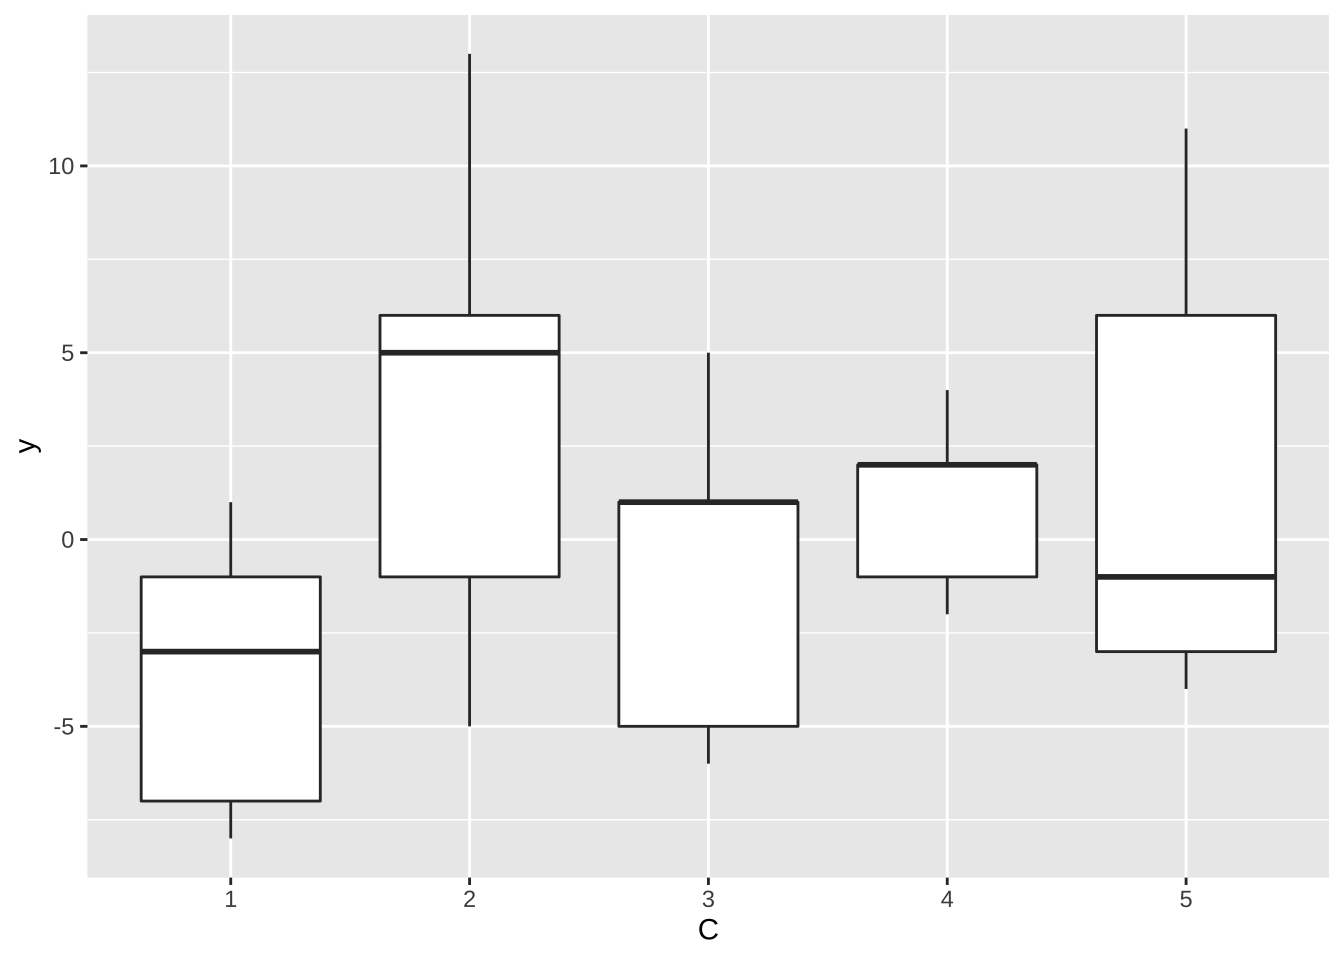
\includegraphics{Two-way-ANOVA_files/figure-latex/unnamed-chunk-15-1.pdf}

\begin{Shaded}
\begin{Highlighting}[]
\NormalTok{df2 }\SpecialCharTok{\%\textgreater{}\%} 
  \FunctionTok{ggplot}\NormalTok{() }\SpecialCharTok{+}
  \FunctionTok{aes}\NormalTok{(}\AttributeTok{x =}\NormalTok{ breed  , }\AttributeTok{y =}\NormalTok{ response, }\AttributeTok{fill=}\NormalTok{food, }\AttributeTok{color=}\NormalTok{food, }\AttributeTok{group =} \FunctionTok{interaction}\NormalTok{(breed,food)) }\SpecialCharTok{+}
  \FunctionTok{geom\_boxplot}\NormalTok{(}\AttributeTok{alpha =} \FloatTok{0.1}\NormalTok{, }\AttributeTok{width =} \FloatTok{0.75}\NormalTok{) }\SpecialCharTok{+}
  \FunctionTok{geom\_beeswarm}\NormalTok{(}\AttributeTok{dodge.width =} \FloatTok{0.75}\NormalTok{)}
\end{Highlighting}
\end{Shaded}

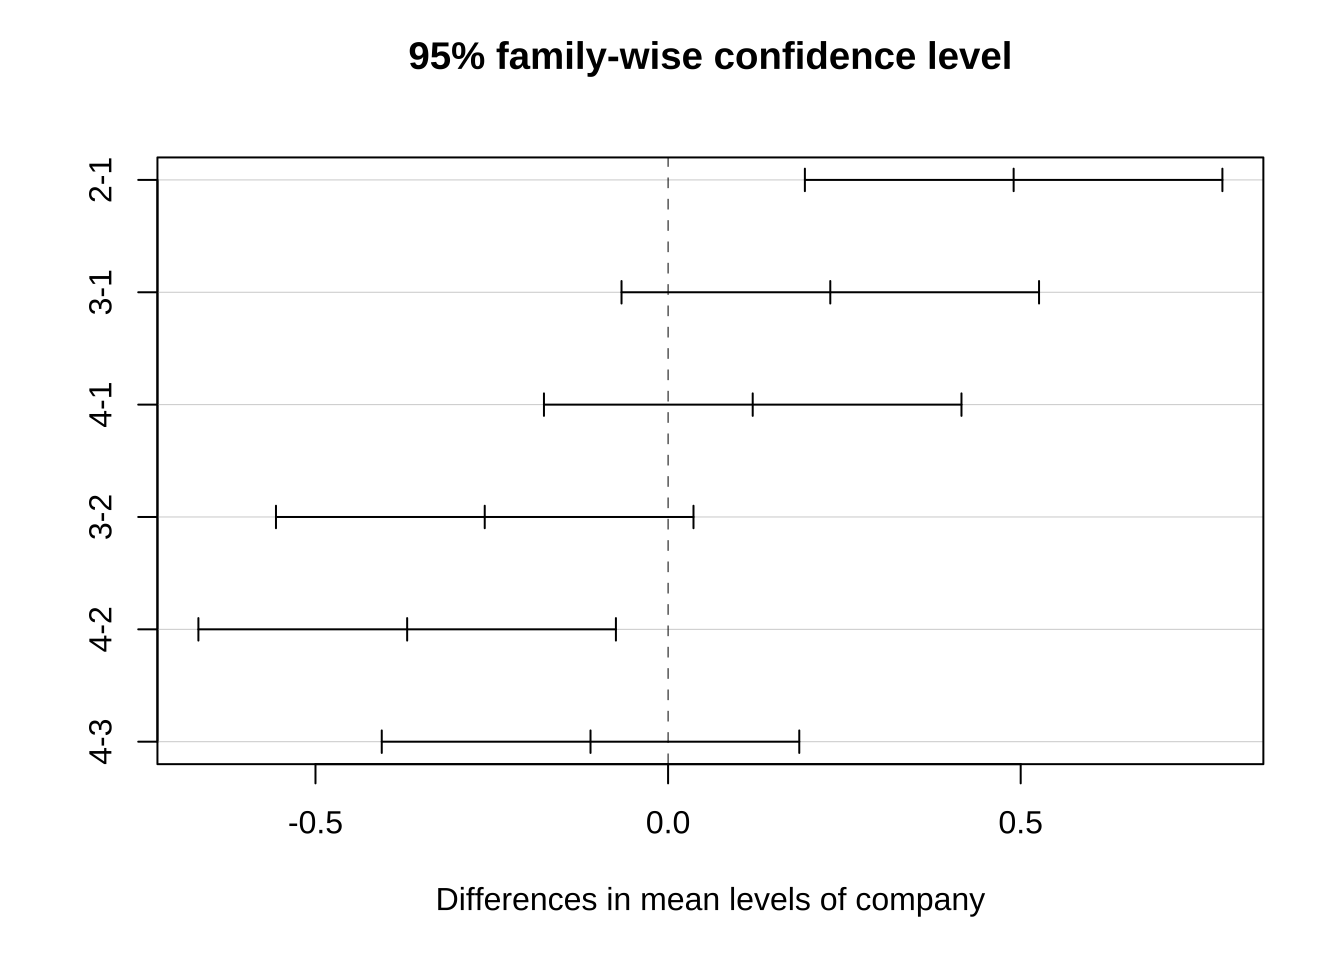
\includegraphics{Two-way-ANOVA_files/figure-latex/unnamed-chunk-16-1.pdf}

위와 같이 두 요인의 조합으로 그림을 보는 것보다 각 요인별로 요약하여 보는 것도 유용하다.

\begin{Shaded}
\begin{Highlighting}[]
\NormalTok{df2 }\SpecialCharTok{\%\textgreater{}\%} 
  \FunctionTok{ggplot}\NormalTok{( }\FunctionTok{aes}\NormalTok{(}\AttributeTok{x =}\NormalTok{ food , }\AttributeTok{y =}\NormalTok{ response) ) }\SpecialCharTok{+}
  \FunctionTok{geom\_boxplot}\NormalTok{()}
\end{Highlighting}
\end{Shaded}

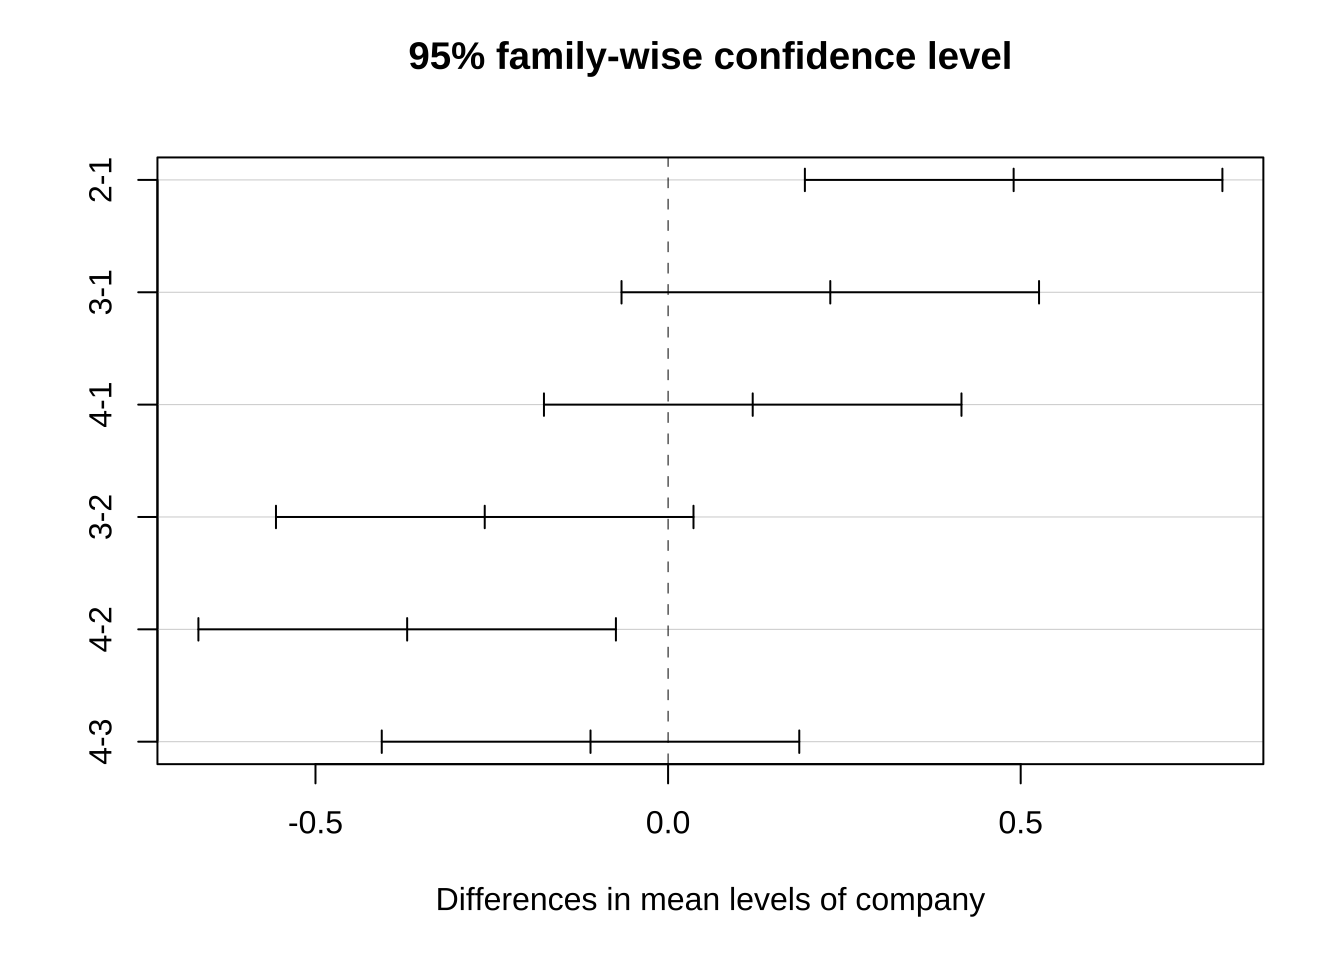
\includegraphics{Two-way-ANOVA_files/figure-latex/unnamed-chunk-17-1.pdf}

\begin{Shaded}
\begin{Highlighting}[]
\NormalTok{df2 }\SpecialCharTok{\%\textgreater{}\%} 
  \FunctionTok{ggplot}\NormalTok{( }\FunctionTok{aes}\NormalTok{(}\AttributeTok{x =}\NormalTok{ breed , }\AttributeTok{y =}\NormalTok{ response))  }\SpecialCharTok{+}
  \FunctionTok{geom\_boxplot}\NormalTok{()}
\end{Highlighting}
\end{Shaded}

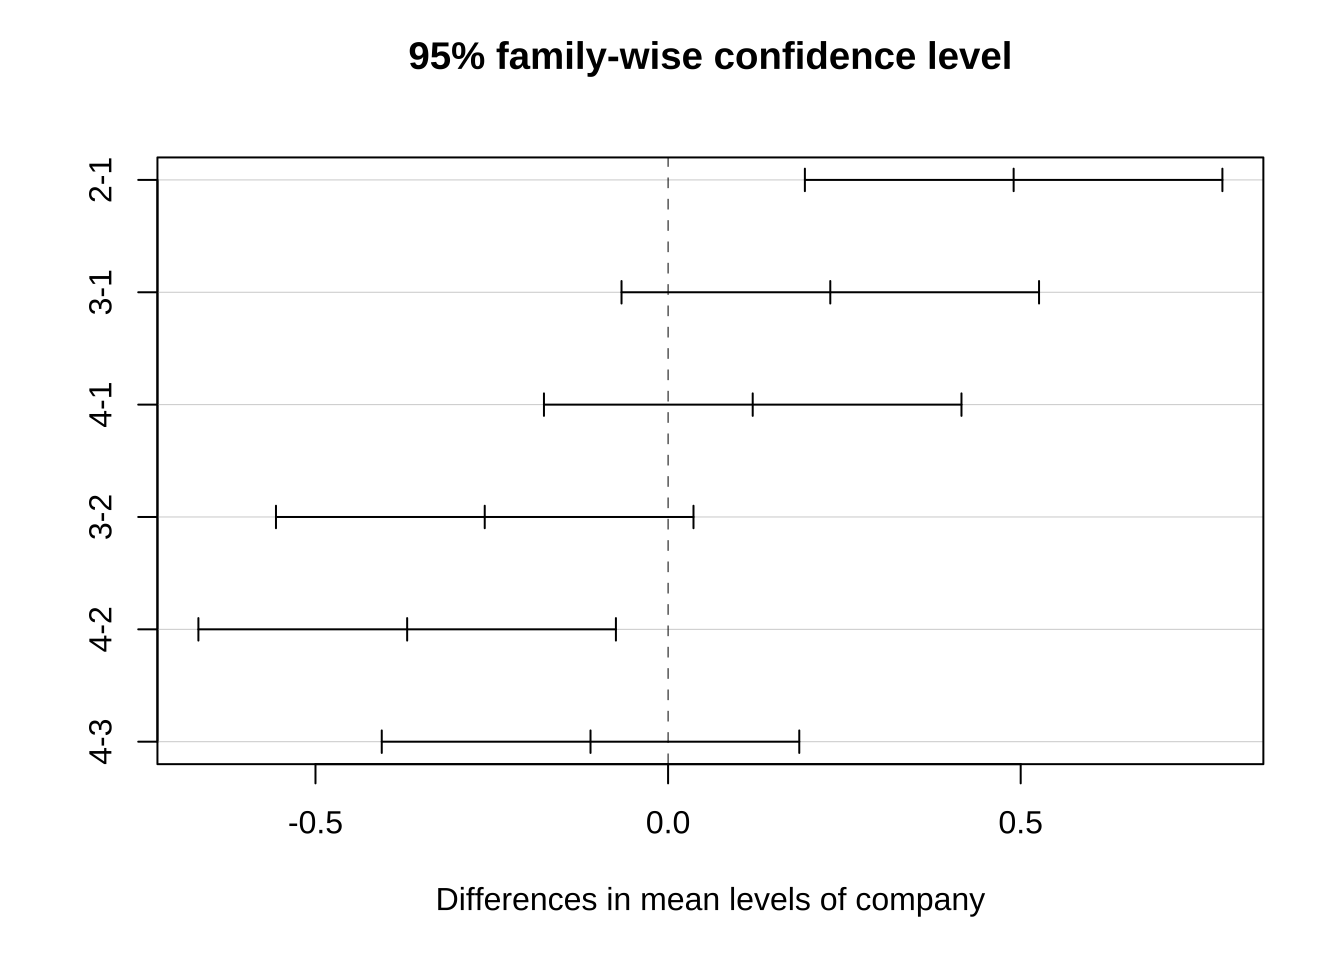
\includegraphics{Two-way-ANOVA_files/figure-latex/unnamed-chunk-18-1.pdf}

다음으로 12개의 처리 조합에 대한 체중의 기초통계량(평균과 표준편차)을 구해보자.

\begin{Shaded}
\begin{Highlighting}[]
\NormalTok{df2s }\OtherTok{\textless{}{-}}\NormalTok{ df2 }\SpecialCharTok{\%\textgreater{}\%} \FunctionTok{group\_by}\NormalTok{(food, breed)  }\SpecialCharTok{\%\textgreater{}\%}  \FunctionTok{summarise}\NormalTok{(}\AttributeTok{mean=}\FunctionTok{mean}\NormalTok{(response),  }\AttributeTok{sd=}\FunctionTok{sd}\NormalTok{(response))}
\end{Highlighting}
\end{Shaded}

\begin{verbatim}
## `summarise()` has grouped output by 'food'. You can override using the `.groups` argument.
\end{verbatim}

\begin{Shaded}
\begin{Highlighting}[]
\NormalTok{df2s}
\end{Highlighting}
\end{Shaded}

\begin{verbatim}
## # A tibble: 12 x 4
## # Groups:   food [4]
##    food  breed  mean    sd
##    <fct> <fct> <dbl> <dbl>
##  1 1     1      66.7  3.06
##  2 1     2      72.3  8.50
##  3 1     3      63.3 11.6 
##  4 2     1      62    3.61
##  5 2     2      50.7  7.09
##  6 2     3      57.3 10.0 
##  7 3     1      64    4.58
##  8 3     2      65.3  6.03
##  9 3     3      46.3 10.2 
## 10 4     1      48.3  8.74
## 11 4     2      57    4   
## 12 4     3      50   10.8
\end{verbatim}

이제 위에서 계산된 처리 그룹에 대한 평균으로 상호작용 그림을 그려보자. 아래 그림에서 사료의 종류에 따라서 체중의 변화를 본 그림이다. 사료 1번에서 체중이 가장 크게 나타났고 다른 사료에 대해서는 체중이 줄어드는데 품종에 따라서 그 크기가 서로 다르다.

\begin{Shaded}
\begin{Highlighting}[]
\NormalTok{df2s }\SpecialCharTok{\%\textgreater{}\%} 
  \FunctionTok{ggplot}\NormalTok{() }\SpecialCharTok{+}
  \FunctionTok{aes}\NormalTok{(}\AttributeTok{x =}\NormalTok{ food , }\AttributeTok{y =}\NormalTok{ mean, }\AttributeTok{color =}\NormalTok{breed) }\SpecialCharTok{+}
  \FunctionTok{geom\_line}\NormalTok{(}\FunctionTok{aes}\NormalTok{(}\AttributeTok{group =}\NormalTok{ breed)) }\SpecialCharTok{+}
  \FunctionTok{geom\_point}\NormalTok{()}
\end{Highlighting}
\end{Shaded}

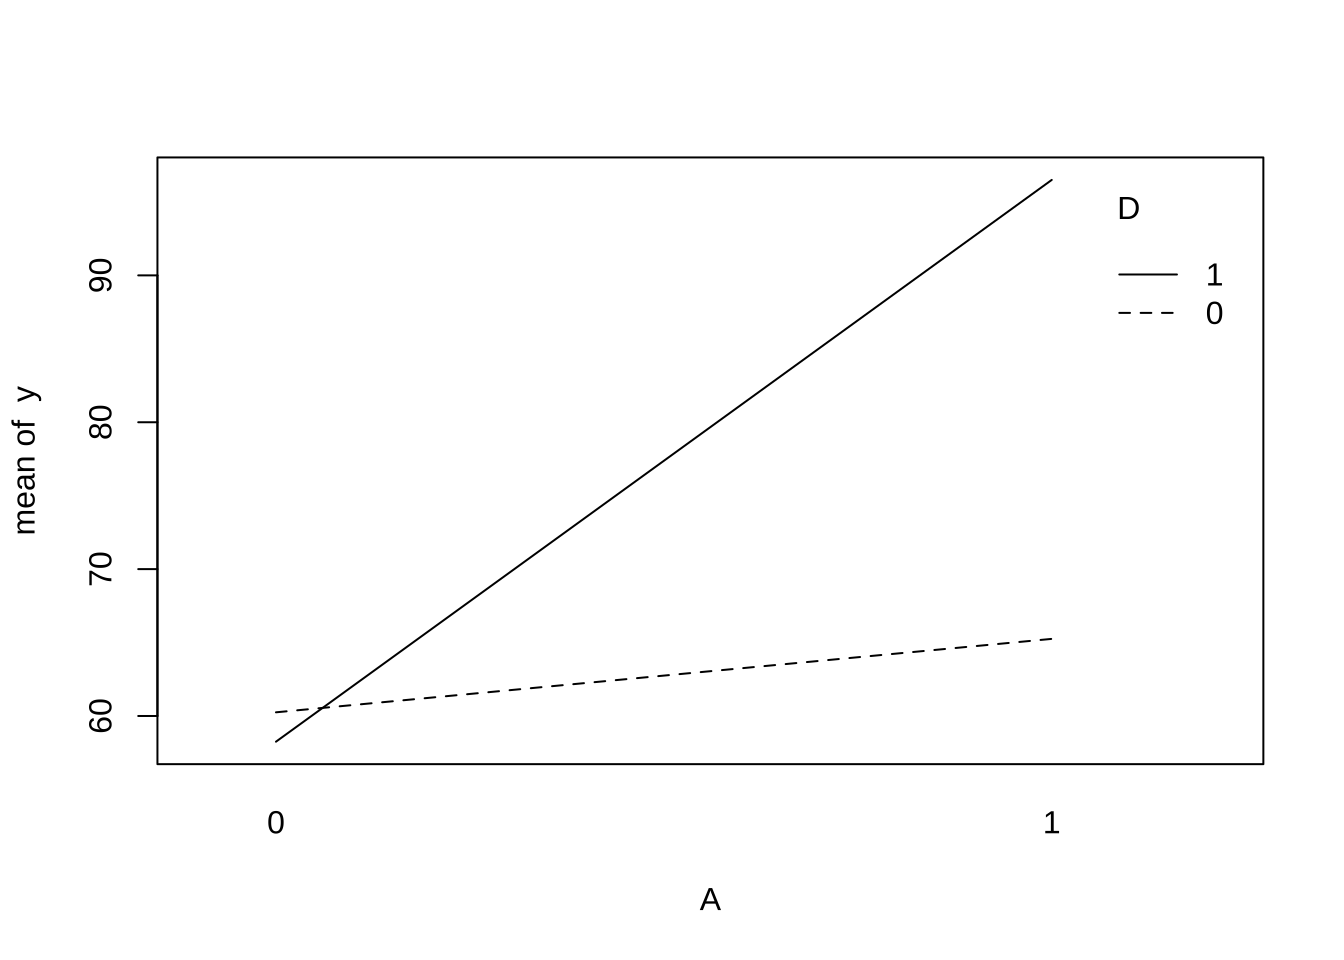
\includegraphics{Two-way-ANOVA_files/figure-latex/unnamed-chunk-20-1.pdf}

아래 그림은 아래 그림에서 품종의 종류에 따라서 체중의 변화를 본 그림이다.

\begin{Shaded}
\begin{Highlighting}[]
\NormalTok{df2s }\SpecialCharTok{\%\textgreater{}\%} 
  \FunctionTok{ggplot}\NormalTok{() }\SpecialCharTok{+}
  \FunctionTok{aes}\NormalTok{(}\AttributeTok{x =}\NormalTok{ breed , }\AttributeTok{y =}\NormalTok{ mean, }\AttributeTok{color =}\NormalTok{food) }\SpecialCharTok{+}
  \FunctionTok{geom\_line}\NormalTok{(}\FunctionTok{aes}\NormalTok{(}\AttributeTok{group =}\NormalTok{ food)) }\SpecialCharTok{+}
  \FunctionTok{geom\_point}\NormalTok{()}
\end{Highlighting}
\end{Shaded}

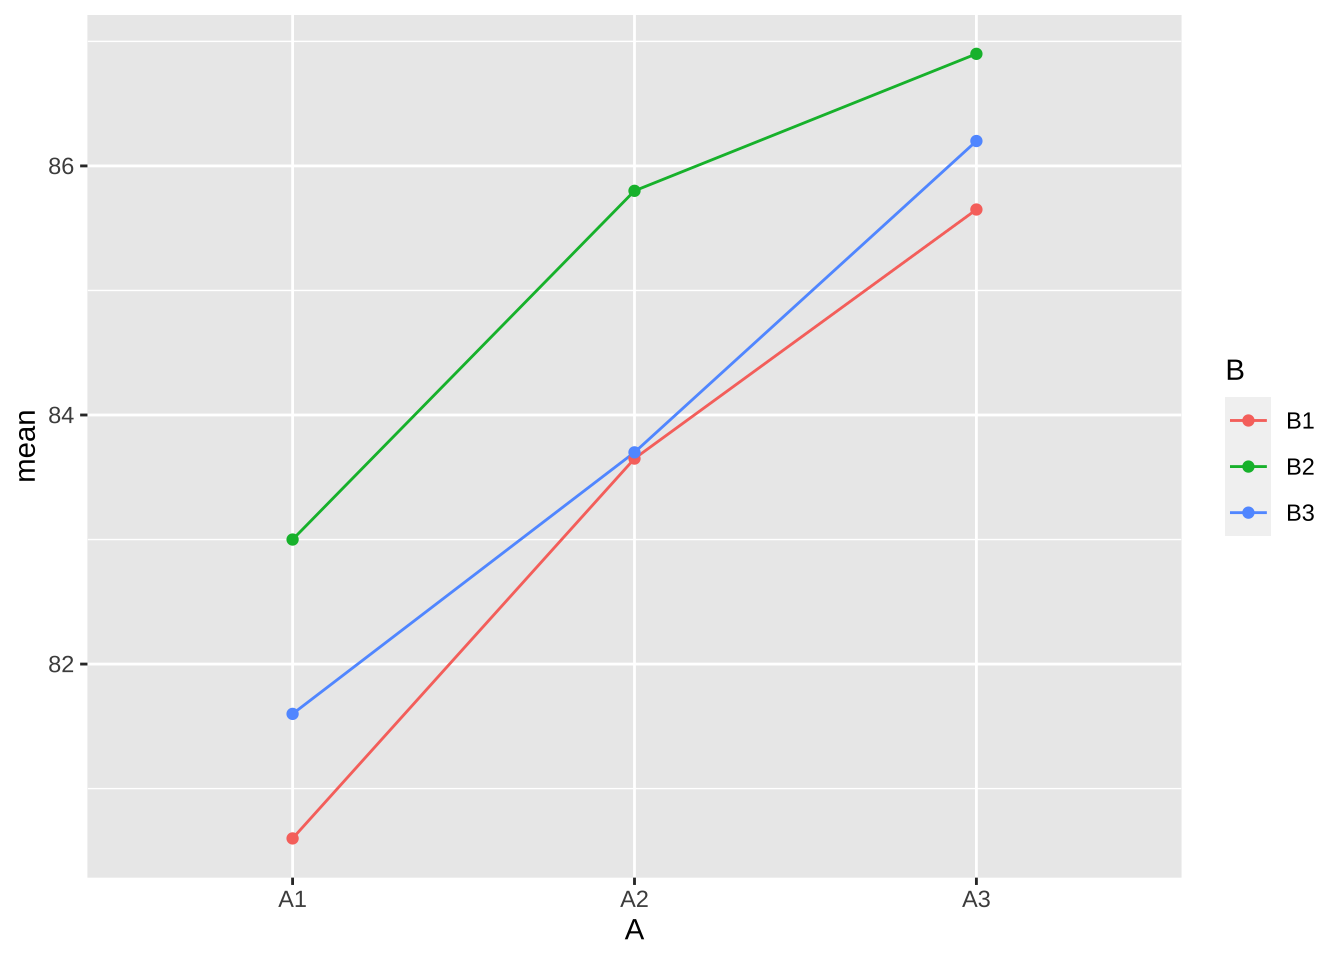
\includegraphics{Two-way-ANOVA_files/figure-latex/unnamed-chunk-21-1.pdf}

사료와 품종간에 상호 작용이 그림으로 나타나고 있지만 뚜렸하지 않고 해석하기도 힘들다.

\hypertarget{uxbd84uxc0b0uxbd84uxc11duxd45cuxc640-uxac00uxc124uxac80uxc815-1}{%
\section{분산분석표와 가설검정}\label{uxbd84uxc0b0uxbd84uxc11duxd45cuxc640-uxac00uxc124uxac80uxc815-1}}

이제 이원배치법에서의 가설검정을 수행하기 위하여 분산분석 표를 구해보자.

\begin{Shaded}
\begin{Highlighting}[]
\NormalTok{df2aov }\OtherTok{\textless{}{-}} \FunctionTok{aov}\NormalTok{(response }\SpecialCharTok{\textasciitilde{}}\NormalTok{ food}\SpecialCharTok{*}\NormalTok{breed, }\AttributeTok{data=}\NormalTok{df2)}
\FunctionTok{summary}\NormalTok{(df2aov)}
\end{Highlighting}
\end{Shaded}

\begin{verbatim}
##             Df Sum Sq Mean Sq F value  Pr(>F)   
## food         3 1156.6   385.5   6.163 0.00294 **
## breed        2  349.4   174.7   2.793 0.08121 . 
## food:breed   6  771.3   128.5   2.055 0.09712 . 
## Residuals   24 1501.3    62.6                   
## ---
## Signif. codes:  0 '***' 0.001 '**' 0.01 '*' 0.05 '.' 0.1 ' ' 1
\end{verbatim}

\begin{itemize}
\item
  상호작용에 대한 가설 검정
  \[ H_0: (\alpha \beta)_{11} = (\alpha \beta)_{12} =\cdots = (\alpha \beta)_{6} =0 \quad \text{ vs.} \quad H_1: \text{ not } H_0 \]

  분산분석표에서 상호작용에 대한 가설 검정을 위한 F-통계량은 \(2.055\)이고 p-값은 0.097으로 유의수준 0.05보다 크므로 귀무가설 \(H_0\)를 기각할 수 있다. 따라서 사료와 품종 간의 상호작용은 유의하지 않다. 하지만 p-값이 0.1 미만이므로 품종에 따라서 사료가 주는 효과가 약간은 다를 가능성이 존재한다.
\end{itemize}

\begin{rmdnote}
상호작용에 대한 p-값이 0.25 보다 작으므로 상호작용에 대한 모수를 가진 모형을 그대로 사용한다. (아래 상호작용이 없는 모형에서의 추론 참조)
\end{rmdnote}
- 주효과에 대한 가설 검정

주효과에 대한 검정에서 품종에 대한 검정은 p-값이 \(0.081\)로서 유의수준 5\%에서 귀무가설을 기각할 수 없으므로 돼지품종에 따라서는 유의한 차이가 없다. 다만 유의수준 1\%에서는 유의하므로 약간의 차이는 있다고 말할 수 있다.

사료에 대한 검정은 p-값이 \(0.003\)로서 유의수준 5\%에서 귀무가설을 기각할 수 있어서 사료에 따라서는 유의한 차이가 있다.

\begin{rmdnote}
보통 유의수준 1\%에서 유의하면 ``\textbf{제한적으로 유의하다}''(marginally significant)라고 말한다.
\end{rmdnote}

\hypertarget{uxbd84uxc0b0uxbd84uxc11d-uxd6c4uxc758-uxcd94uxc815-1}{%
\section{분산분석 후의 추정}\label{uxbd84uxc0b0uxbd84uxc11d-uxd6c4uxc758-uxcd94uxc815-1}}

\hypertarget{uxbaa8uxd3c9uxade0uxc5d0-uxb300uxd55c-uxcd94uxb860-1}{%
\subsection{모평균에 대한 추론}\label{uxbaa8uxd3c9uxade0uxc5d0-uxb300uxd55c-uxcd94uxb860-1}}

이원배치에서 유의한 상호작용이 있는 경우 처리수준 \(A_iB_j\)에 대한 모평균 \(\mu_{ij}\) 에 대한 추정량은 처리수준 \(A_iB_j\)에서의 관측값들의 평균 \(\bar {x}_{ij.}\) 이며 오차항의 분산 \(\sigma^2_E\)는 분산분석표에서 \(MS_E\)로 추정할 수 있다.

\[ \hat \sigma^2_E = MS_E = \frac{SS_E}{ab(r-1)} =\frac{18231}{27} = 675 \]

위의 결과를 이용하면 처리수준 \(A_iB_j\)에 대한 모평균 \(\mu_{ij}\)에 대한 \(100(1-\alpha)\)\% 신뢰구간은 다음과 같이 주어진다.

\[ \bar x_{ij.} \pm t(1-\alpha/2, ab[r-1]) \sqrt{ \frac{MS_E}{r}} \]

예를 들어 사료가 1 이고(\(i=1\)) 품종이 1인 경우(\(j=1\)) 체중의 평균 \(\mu_{11}\) 에 대한 95\% 신뢰 구간을 구해보자. 일단 위의 기초 통계량에서 \(\bar x_{11.}=66.7\) 이고 분산분석표에서 \(MS_E =62.6\), \(r=3\) 그리고 t-분포의 백분위수 \(t(0.975, 24)\) 은 다음과 같이 주어진다.

\begin{Shaded}
\begin{Highlighting}[]
\FunctionTok{qt}\NormalTok{(}\FloatTok{0.975}\NormalTok{, }\DecValTok{24}\NormalTok{)}
\end{Highlighting}
\end{Shaded}

\begin{verbatim}
## [1] 2.063899
\end{verbatim}

따라서 \(\mu_{11}\) 에 대한 95\% 신뢰 구간은 다음과 같다.

\begin{equation}
\bar x_{11.} \pm t(1-\alpha/2, 24) \sqrt{ \frac{MS_E}{r}} = 66.7 \pm (2.06)\sqrt{\frac{62.6}{3}} = (57, 76) 
\label{eq:confint}
\end{equation}

패키지 \texttt{emmeans}에 있는 함수 \texttt{emmeans()}를 다음과 같이 사용하면 각 처리에 대한 평균의 95\% 신뢰구간을 쉽게 구할 수 있다.

\begin{Shaded}
\begin{Highlighting}[]
\FunctionTok{emmeans}\NormalTok{(df2aov, }\StringTok{"food"}\NormalTok{, }\StringTok{"breed"}\NormalTok{)}
\end{Highlighting}
\end{Shaded}

\begin{verbatim}
## breed = 1:
##  food emmean   SE df lower.CL upper.CL
##  1      66.7 4.57 24     57.2     76.1
##  2      62.0 4.57 24     52.6     71.4
##  3      64.0 4.57 24     54.6     73.4
##  4      48.3 4.57 24     38.9     57.8
## 
## breed = 2:
##  food emmean   SE df lower.CL upper.CL
##  1      72.3 4.57 24     62.9     81.8
##  2      50.7 4.57 24     41.2     60.1
##  3      65.3 4.57 24     55.9     74.8
##  4      57.0 4.57 24     47.6     66.4
## 
## breed = 3:
##  food emmean   SE df lower.CL upper.CL
##  1      63.3 4.57 24     53.9     72.8
##  2      57.3 4.57 24     47.9     66.8
##  3      46.3 4.57 24     36.9     55.8
##  4      50.0 4.57 24     40.6     59.4
## 
## Confidence level used: 0.95
\end{verbatim}

\hypertarget{uxbc18uxbcf5uxc774-uxc788uxb294-uxc774uxc6d0uxbc30uxce58uxc5d0uxc11c-uxc0c1uxd638uxc791uxc6a9uxc774-uxc5c6uxb294-uxacbduxc6b0uxc758-uxcd94uxb860}{%
\section{반복이 있는 이원배치에서 상호작용이 없는 경우의 추론}\label{uxbc18uxbcf5uxc774-uxc788uxb294-uxc774uxc6d0uxbc30uxce58uxc5d0uxc11c-uxc0c1uxd638uxc791uxc6a9uxc774-uxc5c6uxb294-uxacbduxc6b0uxc758-uxcd94uxb860}}

교과서에서 상호작용의 유의성에 따라서 모형을 축소하는 기준을 다음과 같이 제시하고 있다.

상호작용에 대한 p-값이 0.25보다 큰 경우 상호작용이 존재하지 않는다고 판단하고 오차항에 풀링힌다. 상호작용을 오차항에 풀링한다는 것은 다음과 같은 모형을 사용한다는 의미이다.

\begin{equation}
 x_{ijk} = \mu + \alpha_i + \beta_j + e_{ijk} 
\label{eq:nointer}
\end{equation}

만약 예제 4.1에 대한 반복이 있는 자료에서 위와 같이 오차항을 풀링한 모형을 적합해 보면 아래와 같은 분산분석표를 얻는다.

\begin{Shaded}
\begin{Highlighting}[]
\NormalTok{df2aov2 }\OtherTok{\textless{}{-}} \FunctionTok{aov}\NormalTok{(response }\SpecialCharTok{\textasciitilde{}}\NormalTok{ food }\SpecialCharTok{+}\NormalTok{ breed, }\AttributeTok{data=}\NormalTok{df2)}
\FunctionTok{summary}\NormalTok{(df2aov2)}
\end{Highlighting}
\end{Shaded}

\begin{verbatim}
##             Df Sum Sq Mean Sq F value  Pr(>F)   
## food         3 1156.6   385.5   5.089 0.00575 **
## breed        2  349.4   174.7   2.306 0.11705   
## Residuals   30 2272.6    75.8                   
## ---
## Signif. codes:  0 '***' 0.001 '**' 0.01 '*' 0.05 '.' 0.1 ' ' 1
\end{verbatim}

만약 \textbf{반복이 있는 이원배치 모형}에서 상호작용 \(A \times B\)가 존재하지 않고 주효과만 유의한 경우, 즉 모형 \eqref{eq:nointer}을 가정한 경우 모평균 \(\mu_{ij}\)에 대한 모수는 다음과 같다.

\[ \mu_{ij} = \mu + \alpha_i + \beta_j \]

이러한 경우 모평균 \(\mu_{ij}\)에 대한 최소제곱 추정량(least square estimator)은 표본 평균 \(\bar x_{ij.}\)이 아니라 다음과 같은 추정량이 주어진다.

\begin{align*}
\hat \mu_{ij} & = \hat \mu + \hat \alpha_i + \hat \beta_j \\
  & = (\bar{\bar x}) + (\bar x_{i..}-\bar{\bar x}) + (\bar x_{.j.}-\bar{\bar x}) \\
  & = \bar x_{i..} + \bar x_{.j.} - \bar{\bar x} 
\end{align*}

위에서 주어진 \(\hat \mu_{ij}\) 는 모평균 \(\mu_{ij}\)의 불편 추정량이며 상호작용 \(A \times B\) 이 없는 모형 \eqref{eq:nointer} 에서 표본 평균 \(\bar x_{ij.}\) 보다 분산이 작은 추정량이다. 즉,

\[ Var \left (\hat \mu_{ij} \right ) = \frac{\sigma_E^2}{n_e}  \le \frac{\sigma_E^2}{r} = Var (\bar x_{ij.} )    \]

위의 식에서 유효 반복수 \(n_e\) 는 다음과 같이 정의된다.

\[ \frac{1}{n_e} = \frac{1}{br} + \frac{1}{ar} - \frac{1}{abr}, \quad n_e=\frac{abr}{a+b-1} \]

따라서 이 경우 모평균 \(\mu_{ij}\)에 대한 \(100(1-\alpha)\)\% 신뢰구간은 다음과 같은 주어진다.

\[ \hat \mu_{ij} \pm t(1-\alpha/2, \phi_E) \sqrt{ \frac{MS_E}{n_e}} \]

주의할 점은 위의 신뢰구간에서 \(MS_E\)는 상호작용이 없는 모형 \eqref{eq:nointer} 으로 유도된 분산분석표에 나타난 \(MS_E\) 이며 자유도는 \(\phi_E = abr-a-b+1\) 이다.

참고로 예제 4.1 경우 \(a=4\), \(b=3\), \(r=3\)이므로 유효 반복수 \(n_e\) 는 다음과 같이 주어진다.

\[ n_e = \frac{abr}{a+b-1} = \frac{(4)(3)(3)}{4+3-1} = 6  \]

상호작용 \(A \times B\) 이 없는 모형 \eqref{eq:nointer} 에서 적용한 분산분석 결과\texttt{df2aov2} 에 대하여 함수 \texttt{emmeans()}를 다음과 같이 사용하면 모형 \eqref{eq:nointer} 에서 각 처리에 대한 평균 \(\mu_{ij}\)에 대한 최소제곱 추정량 \(\hat \mu_{ij}=\bar x_{i..} + \bar x_{.j.} - \bar{\bar x}\) 과 95\% 신뢰구간을 다음과 같이 구할 수 있다.

\begin{Shaded}
\begin{Highlighting}[]
\FunctionTok{emmeans}\NormalTok{(df2aov2, }\StringTok{"food"}\NormalTok{, }\StringTok{"breed"}\NormalTok{)}
\end{Highlighting}
\end{Shaded}

\begin{verbatim}
## breed = 1:
##  food emmean   SE df lower.CL upper.CL
##  1      69.1 3.55 30     61.8     76.3
##  2      58.3 3.55 30     51.0     65.6
##  3      60.2 3.55 30     52.9     67.5
##  4      53.4 3.55 30     46.2     60.7
## 
## breed = 2:
##  food emmean   SE df lower.CL upper.CL
##  1      70.2 3.55 30     62.9     77.4
##  2      59.4 3.55 30     52.1     66.6
##  3      61.3 3.55 30     54.0     68.5
##  4      54.5 3.55 30     47.2     61.8
## 
## breed = 3:
##  food emmean   SE df lower.CL upper.CL
##  1      63.1 3.55 30     55.8     70.3
##  2      52.3 3.55 30     45.0     59.6
##  3      54.2 3.55 30     46.9     61.5
##  4      47.4 3.55 30     40.2     54.7
## 
## Confidence level used: 0.95
\end{verbatim}

위에서 나타난 \texttt{emmean} 은 \(\mu_{ij}\)에 대한 최소제곱 추정량 \(\bar x_{i..} + \bar x_{.j.} - \bar{\bar x}\) 으로서 아래 주어진 표본평균 \(\bar x_{ij.}\) 과 다른 값으로 나타남을 알 수 있다.

\begin{Shaded}
\begin{Highlighting}[]
\NormalTok{df2s}
\end{Highlighting}
\end{Shaded}

\begin{verbatim}
## # A tibble: 12 x 4
## # Groups:   food [4]
##    food  breed  mean    sd
##    <fct> <fct> <dbl> <dbl>
##  1 1     1      66.7  3.06
##  2 1     2      72.3  8.50
##  3 1     3      63.3 11.6 
##  4 2     1      62    3.61
##  5 2     2      50.7  7.09
##  6 2     3      57.3 10.0 
##  7 3     1      64    4.58
##  8 3     2      65.3  6.03
##  9 3     3      46.3 10.2 
## 10 4     1      48.3  8.74
## 11 4     2      57    4   
## 12 4     3      50   10.8
\end{verbatim}

예를 들어 상호작용 \(A \times B\) 이 없는 모형 \eqref{eq:nointer} 에서 \(\mu_{11}\) 에 대한 95\% 신뢰 구간은 다음과 같다.

\begin{align*}
\hat \mu_{11}  \pm t(1-\alpha/2, 30) \sqrt{ \frac{MS_E}{n_e}} 
& = 69.1 \pm (2.04)\sqrt{\frac{ 75.8}{6}} \\
& = 69.1 \pm (2.04)(3.55) \\
& = (61.8, 76.3) 
\end{align*}

위의 신뢰구간 \((61.8, 76.3)\)은 상호 작용이 포함된 모형에서 유도힌 신뢰구간 \eqref{eq:confint}에서 구한 \((57, 76)\)과 다르다.

  \bibliography{book.bib,packages.bib}

\end{document}
